\begin{frame}
  \footnotesize

  \begin{figure}[h]\centering\vspace{1cm}
     \begin{subfigure}{0.49\linewidth}\centering
       % GNUPLOT: LaTeX picture with Postscript
\begingroup
  \makeatletter
  \providecommand\color[2][]{%
    \GenericError{(gnuplot) \space\space\space\@spaces}{%
      Package color not loaded in conjunction with
      terminal option `colourtext'%
    }{See the gnuplot documentation for explanation.%
    }{Either use 'blacktext' in gnuplot or load the package
      color.sty in LaTeX.}%
    \renewcommand\color[2][]{}%
  }%
  \providecommand\includegraphics[2][]{%
    \GenericError{(gnuplot) \space\space\space\@spaces}{%
      Package graphicx or graphics not loaded%
    }{See the gnuplot documentation for explanation.%
    }{The gnuplot epslatex terminal needs graphicx.sty or graphics.sty.}%
    \renewcommand\includegraphics[2][]{}%
  }%
  \providecommand\rotatebox[2]{#2}%
  \@ifundefined{ifGPcolor}{%
    \newif\ifGPcolor
    \GPcolorfalse
  }{}%
  \@ifundefined{ifGPblacktext}{%
    \newif\ifGPblacktext
    \GPblacktexttrue
  }{}%
  % define a \g@addto@macro without @ in the name:
  \let\gplgaddtomacro\g@addto@macro
  % define empty templates for all commands taking text:
  \gdef\gplfronttext{}%
  \gdef\gplfronttext{}%
  \makeatother
  \ifGPblacktext
    % no textcolor at all
    \def\colorrgb#1{}%
    \def\colorgray#1{}%
  \else
    % gray or color?
    \ifGPcolor
      \def\colorrgb#1{\color[rgb]{#1}}%
      \def\colorgray#1{\color[gray]{#1}}%
      \expandafter\def\csname LTw\endcsname{\color{white}}%
      \expandafter\def\csname LTb\endcsname{\color{black}}%
      \expandafter\def\csname LTa\endcsname{\color{black}}%
      \expandafter\def\csname LT0\endcsname{\color[rgb]{1,0,0}}%
      \expandafter\def\csname LT1\endcsname{\color[rgb]{0,1,0}}%
      \expandafter\def\csname LT2\endcsname{\color[rgb]{0,0,1}}%
      \expandafter\def\csname LT3\endcsname{\color[rgb]{1,0,1}}%
      \expandafter\def\csname LT4\endcsname{\color[rgb]{0,1,1}}%
      \expandafter\def\csname LT5\endcsname{\color[rgb]{1,1,0}}%
      \expandafter\def\csname LT6\endcsname{\color[rgb]{0,0,0}}%
      \expandafter\def\csname LT7\endcsname{\color[rgb]{1,0.3,0}}%
      \expandafter\def\csname LT8\endcsname{\color[rgb]{0.5,0.5,0.5}}%
    \else
      % gray
      \def\colorrgb#1{\color{black}}%
      \def\colorgray#1{\color[gray]{#1}}%
      \expandafter\def\csname LTw\endcsname{\color{white}}%
      \expandafter\def\csname LTb\endcsname{\color{black}}%
      \expandafter\def\csname LTa\endcsname{\color{black}}%
      \expandafter\def\csname LT0\endcsname{\color{black}}%
      \expandafter\def\csname LT1\endcsname{\color{black}}%
      \expandafter\def\csname LT2\endcsname{\color{black}}%
      \expandafter\def\csname LT3\endcsname{\color{black}}%
      \expandafter\def\csname LT4\endcsname{\color{black}}%
      \expandafter\def\csname LT5\endcsname{\color{black}}%
      \expandafter\def\csname LT6\endcsname{\color{black}}%
      \expandafter\def\csname LT7\endcsname{\color{black}}%
      \expandafter\def\csname LT8\endcsname{\color{black}}%
    \fi
  \fi
  \setlength{\unitlength}{0.0500bp}%
  \begin{picture}(4000.00,3200.00)%
    \gplgaddtomacro\gplfronttext{%
      \colorrgb{0.00,0.00,0.00}%
      \put(726,440){\makebox(0,0)[r]{\strut{}$0.0$}}%
      \colorrgb{0.00,0.00,0.00}%
      \put(726,752){\makebox(0,0)[r]{\strut{}$0.01$}}%
      \colorrgb{0.00,0.00,0.00}%
      \put(726,1064){\makebox(0,0)[r]{\strut{}$0.02$}}%
      \colorrgb{0.00,0.00,0.00}%
      \put(726,1376){\makebox(0,0)[r]{\strut{}$0.03$}}%
      \colorrgb{0.00,0.00,0.00}%
      \put(726,1688){\makebox(0,0)[r]{\strut{}$0.04$}}%
      \colorrgb{0.00,0.00,0.00}%
      \put(726,1999){\makebox(0,0)[r]{\strut{}$0.05$}}%
      \colorrgb{0.00,0.00,0.00}%
      \put(726,2311){\makebox(0,0)[r]{\strut{}$0.06$}}%
      \colorrgb{0.00,0.00,0.00}%
      \put(726,2623){\makebox(0,0)[r]{\strut{}$0.07$}}%
      \colorrgb{0.00,0.00,0.00}%
      \put(726,2935){\makebox(0,0)[r]{\strut{}$0.08$}}%
      \colorrgb{0.00,0.00,0.00}%
      \put(858,220){\makebox(0,0){\strut{}$0$}}%
      \colorrgb{0.00,0.00,0.00}%
      \put(1316,220){\makebox(0,0){\strut{}$20$}}%
      \colorrgb{0.00,0.00,0.00}%
      \put(1773,220){\makebox(0,0){\strut{}$40$}}%
      \colorrgb{0.00,0.00,0.00}%
      \put(2231,220){\makebox(0,0){\strut{}$60$}}%
      \colorrgb{0.00,0.00,0.00}%
      \put(2688,220){\makebox(0,0){\strut{}$80$}}%
      \colorrgb{0.00,0.00,0.00}%
      \put(3146,220){\makebox(0,0){\strut{}$100$}}%
      \colorrgb{0.00,0.00,0.00}%
      \put(3603,220){\makebox(0,0){\strut{}$120$}}%
      \put(4400,3420){\makebox(0,0){\strut{}Σφάλμα κατάστασης $[(\text{m}^2 + \text{rad}^2)^{1/2}]$}}%
      \put(4400,-200){\makebox(0,0){\strut{}Αριθμός εκτιμήσεων στάσης στο χρόνο}}%
    }%
    \gplgaddtomacro\gplfronttext{%
    }%
    \gplfronttext
    \put(0,0){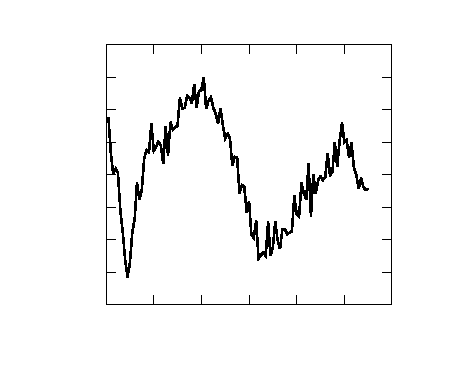
\includegraphics{./figures/parts/02/chapters/01/sections/05/pose_navfn_corridor}}%
    \gplfronttext
  \end{picture}%
\endgroup

     \end{subfigure}
     \begin{subfigure}{0.49\linewidth} \centering
       % GNUPLOT: LaTeX picture with Postscript
\begingroup
  \makeatletter
  \providecommand\color[2][]{%
    \GenericError{(gnuplot) \space\space\space\@spaces}{%
      Package color not loaded in conjunction with
      terminal option `colourtext'%
    }{See the gnuplot documentation for explanation.%
    }{Either use 'blacktext' in gnuplot or load the package
      color.sty in LaTeX.}%
    \renewcommand\color[2][]{}%
  }%
  \providecommand\includegraphics[2][]{%
    \GenericError{(gnuplot) \space\space\space\@spaces}{%
      Package graphicx or graphics not loaded%
    }{See the gnuplot documentation for explanation.%
    }{The gnuplot epslatex terminal needs graphicx.sty or graphics.sty.}%
    \renewcommand\includegraphics[2][]{}%
  }%
  \providecommand\rotatebox[2]{#2}%
  \@ifundefined{ifGPcolor}{%
    \newif\ifGPcolor
    \GPcolorfalse
  }{}%
  \@ifundefined{ifGPblacktext}{%
    \newif\ifGPblacktext
    \GPblacktexttrue
  }{}%
  % define a \g@addto@macro without @ in the name:
  \let\gplgaddtomacro\g@addto@macro
  % define empty templates for all commands taking text:
  \gdef\gplfronttext{}%
  \gdef\gplfronttext{}%
  \makeatother
  \ifGPblacktext
    % no textcolor at all
    \def\colorrgb#1{}%
    \def\colorgray#1{}%
  \else
    % gray or color?
    \ifGPcolor
      \def\colorrgb#1{\color[rgb]{#1}}%
      \def\colorgray#1{\color[gray]{#1}}%
      \expandafter\def\csname LTw\endcsname{\color{white}}%
      \expandafter\def\csname LTb\endcsname{\color{black}}%
      \expandafter\def\csname LTa\endcsname{\color{black}}%
      \expandafter\def\csname LT0\endcsname{\color[rgb]{1,0,0}}%
      \expandafter\def\csname LT1\endcsname{\color[rgb]{0,1,0}}%
      \expandafter\def\csname LT2\endcsname{\color[rgb]{0,0,1}}%
      \expandafter\def\csname LT3\endcsname{\color[rgb]{1,0,1}}%
      \expandafter\def\csname LT4\endcsname{\color[rgb]{0,1,1}}%
      \expandafter\def\csname LT5\endcsname{\color[rgb]{1,1,0}}%
      \expandafter\def\csname LT6\endcsname{\color[rgb]{0,0,0}}%
      \expandafter\def\csname LT7\endcsname{\color[rgb]{1,0.3,0}}%
      \expandafter\def\csname LT8\endcsname{\color[rgb]{0.5,0.5,0.5}}%
    \else
      % gray
      \def\colorrgb#1{\color{black}}%
      \def\colorgray#1{\color[gray]{#1}}%
      \expandafter\def\csname LTw\endcsname{\color{white}}%
      \expandafter\def\csname LTb\endcsname{\color{black}}%
      \expandafter\def\csname LTa\endcsname{\color{black}}%
      \expandafter\def\csname LT0\endcsname{\color{black}}%
      \expandafter\def\csname LT1\endcsname{\color{black}}%
      \expandafter\def\csname LT2\endcsname{\color{black}}%
      \expandafter\def\csname LT3\endcsname{\color{black}}%
      \expandafter\def\csname LT4\endcsname{\color{black}}%
      \expandafter\def\csname LT5\endcsname{\color{black}}%
      \expandafter\def\csname LT6\endcsname{\color{black}}%
      \expandafter\def\csname LT7\endcsname{\color{black}}%
      \expandafter\def\csname LT8\endcsname{\color{black}}%
    \fi
  \fi
  \setlength{\unitlength}{0.0500bp}%
  \begin{picture}(4000.00,3200.00)%
    \gplgaddtomacro\gplfronttext{%
      \colorrgb{0.00,0.00,0.00}%
      \put(726,440){\makebox(0,0)[r]{\strut{}$0.0$}}%
      \colorrgb{0.00,0.00,0.00}%
      \put(726,796){\makebox(0,0)[r]{\strut{}$0.05$}}%
      \colorrgb{0.00,0.00,0.00}%
      \put(726,1153){\makebox(0,0)[r]{\strut{}$0.10$}}%
      \colorrgb{0.00,0.00,0.00}%
      \put(726,1509){\makebox(0,0)[r]{\strut{}$0.15$}}%
      \colorrgb{0.00,0.00,0.00}%
      \put(726,1866){\makebox(0,0)[r]{\strut{}$0.20$}}%
      \colorrgb{0.00,0.00,0.00}%
      \put(726,2222){\makebox(0,0)[r]{\strut{}$0.25$}}%
      \colorrgb{0.00,0.00,0.00}%
      \put(726,2579){\makebox(0,0)[r]{\strut{}$0.30$}}%
      \colorrgb{0.00,0.00,0.00}%
      \put(726,2935){\makebox(0,0)[r]{\strut{}$0.35$}}%
      \colorrgb{0.00,0.00,0.00}%
      \put(858,220){\makebox(0,0){\strut{}$0$}}%
      \colorrgb{0.00,0.00,0.00}%
      \put(1544,220){\makebox(0,0){\strut{}$50$}}%
      \colorrgb{0.00,0.00,0.00}%
      \put(2231,220){\makebox(0,0){\strut{}$100$}}%
      \colorrgb{0.00,0.00,0.00}%
      \put(2917,220){\makebox(0,0){\strut{}$150$}}%
      \colorrgb{0.00,0.00,0.00}%
      \put(3603,220){\makebox(0,0){\strut{}$200$}}%
    }%
    \gplgaddtomacro\gplfronttext{%
    }%
    \put(0,0){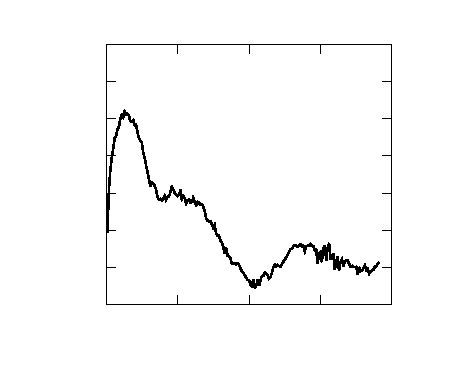
\includegraphics{./figures/parts/02/chapters/01/sections/05/pose_globalplanner_willowgarage}}%
    \gplfronttext
  \end{picture}%
\endgroup

     \end{subfigure}
     \vspace{0.75cm}
  \caption{Μέσος όρος σφαλμάτων εκτίμησης στάσης κατά τη διάρκεια του
           χρόνου σε δέκα πειράματα αυτόνομους πλοήγησης με τη χρήση φίλτρου
           σωματιδίων στα προσομειωμένα περιβάλλοντα CORRIDOR και WILLOWGARAGE}
  \end{figure}


\note{\footnotesize Κατά τη διάρκεια διεξαγωγής της πειραματικής διαδικασίας
  αυτό που παρατήρησα ήταν ότι η εκτίμηση της στάσης εμφάνιζε σφάλματα
  παρατηρήσιμα ακόμα και με γυμνό μάτι. Σε αυτή τη διαφάνεια βλέπουμε την
  εξέλιξη του μέσου σφάλματος εκτίμησης στάσης στα δύο προσομοιωμένα
  περιβάλλοντα, το οποίο δεν εμφανίζει σταθερό μέτρο είτε στην πορεία του
  χρόνου είτε ανά περιβάλλον.  Το μέτρο του σφάλματος εδώ μετριέται σε εκατοστά
  γιατί η στάση του ρομπότ υπόκειται σε εκτίμηση και όχι μέτρηση, δηλαδή
  υποθέτουμε ότι στο περιβάλλον που κινείται το ρομπότ δεν υπάρχει μετρητικός
  εξοπλισμός, αλλά το ρομπότ εκτίμα το ίδιο τη στάση του μέσω των αισθητήρων
  του.}


\end{frame}
